%==============================================================================
%  Problem 1.B -- two-mass system schematic.
%
%  Redrawn from the textbook scan so the labels are text: edit a name here and
%  rebuild with `make`, which exports this file to figures/2_B_Schematic.pdf.
%  The standalone class crops the page to the drawing, so \answerfigure scales
%  it with no stray margin.
%==============================================================================
\documentclass[border=4pt]{standalone}
\usepackage{amsmath}
\usepackage{tikz}
\usetikzlibrary{decorations.pathmorphing,patterns,arrows.meta,calc}

\begin{document}
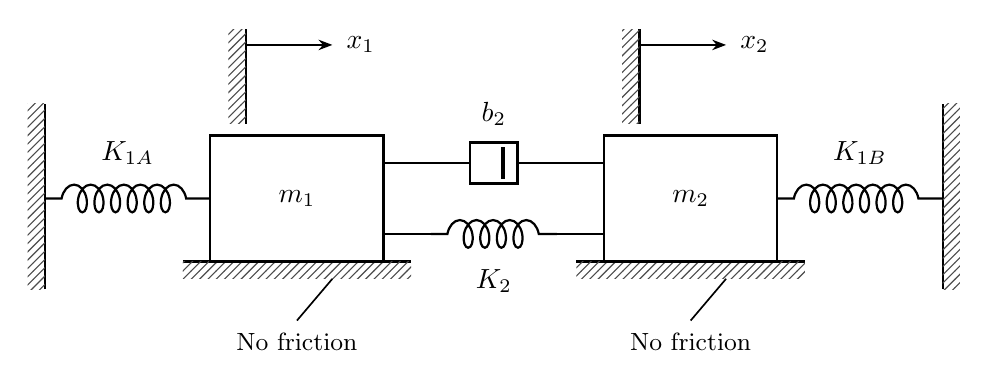
\begin{tikzpicture}[
  line width=0.8pt,
  % A spring is a coil decoration; aspect controls how round the loops look.
  spring/.style={decorate,decoration={coil,amplitude=5pt,segment length=6pt,
                                      aspect=0.6,pre length=6pt,post length=6pt}},
  % Hatching for anything rigidly fixed to ground: walls, ceilings, floors.
  hatch/.style={pattern=north east lines,pattern color=black!70,draw=none},
  mass/.style={draw,fill=white,minimum width=22mm,minimum height=16mm},
  lbl/.style={font=\normalsize},
]

%--- geometry ----------------------------------------------------------------
\def\ybase{0}          % floor / bottom of the masses
\def\ytop{1.6}         % top of the masses
\def\ymid{0.8}         % centre line, where the outer springs attach
\def\hatchw{0.22}      % thickness of a hatched band

\def\xwallL{0}         % inner face of the left wall
\def\xmoneL{2.1}       % left face of m_1
\def\xmoneR{4.3}       % right face of m_1
\def\xmtwoL{7.1}       % left face of m_2
\def\xmtwoR{9.3}       % right face of m_2
\def\xwallR{11.4}      % inner face of the right wall

%--- fixed walls, left and right ---------------------------------------------
\foreach \x/\dir in {\xwallL/-1, \xwallR/1} {
  \draw (\x,-0.35) -- (\x,2.0);
  \fill[hatch] (\x,-0.35) rectangle ($(\x,2.0)+(\dir*\hatchw,0)$);
}

%--- frictionless ground under each mass -------------------------------------
\foreach \xa/\xb in {1.75/4.65, 6.75/9.65} {
  \draw (\xa,\ybase) -- (\xb,\ybase);
  \fill[hatch] (\xa,\ybase) rectangle (\xb,-\hatchw);
}

%--- the two masses ----------------------------------------------------------
\node[mass] (m1) at ($0.5*(\xmoneL,0)+0.5*(\xmoneR,0)+(0,\ymid)$) {$m_1$};
\node[mass] (m2) at ($0.5*(\xmtwoL,0)+0.5*(\xmtwoR,0)+(0,\ymid)$) {$m_2$};

%--- outer springs: K_{1A} on the left, K_{1B} on the right ------------------
\draw[spring] (\xwallL,\ymid) -- (\xmoneL,\ymid);
\node[lbl,above] at (1.05,\ymid+0.30) {$K_{1A}$};

\draw[spring] (\xmtwoR,\ymid) -- (\xwallR,\ymid);
\node[lbl,above] at (10.35,\ymid+0.30) {$K_{1B}$};

%--- coupling: shock absorber b_2 above, spring K_2 below --------------------
\def\ydash{1.25}       % height of the dashpot run
\def\yktwo{0.35}       % height of the inner spring run
\def\xdashc{5.7}       % centre of the dashpot body

% Dashpot: cylinder open towards m_1, plunger rod entering from m_2.
\draw (\xmoneR,\ydash) -- ($(\xdashc,\ydash)-(0.30,0)$);
\draw ($(\xdashc,\ydash)+(0.30,0)$) -- (\xmtwoL,\ydash);
\draw ($(\xdashc,\ydash)+(-0.30,-0.26)$) rectangle ($(\xdashc,\ydash)+(0.30,0.26)$);
\draw[line width=1.4pt] ($(\xdashc,\ydash)+(0.12,-0.20)$) -- ($(\xdashc,\ydash)+(0.12,0.20)$);
\node[lbl,above] at (\xdashc,\ydash+0.34) {$b_2$};

% Inner spring, with a straight lead-in at each end so it clears the masses.
\draw (\xmoneR,\yktwo) -- (4.9,\yktwo);
\draw[spring] (4.9,\yktwo) -- (6.5,\yktwo);
\draw (6.5,\yktwo) -- (\xmtwoL,\yktwo);
\node[lbl,below] at (5.7,\yktwo-0.32) {$K_2$};

%--- displacement references, fixed above each mass --------------------------
% Hatched post = the inertial reference the displacement is measured from;
% the arrow just fixes the positive direction.
\foreach \x/\name in {2.55/{x_1}, 7.55/{x_2}} {
  \draw (\x,\ytop+0.15) -- (\x,\ytop+1.35);
  \fill[hatch] (\x,\ytop+0.15) rectangle ($(\x,\ytop+1.35)-(\hatchw,0)$);
  \draw[-{Stealth[length=5pt]}] (\x,\ytop+1.15) -- ($(\x,\ytop+1.15)+(1.1,0)$);
  \node[lbl,right] at ($(\x,\ytop+1.15)+(1.15,0)$) {$\name$};
}

%--- callouts ----------------------------------------------------------------
\foreach \xm in {3.2, 8.2} {
  \draw[line width=0.6pt] (\xm,-0.75) -- ($(\xm,-\hatchw)-(-0.45,0)$);
  \node[font=\small,below] at (\xm,-0.78) {No friction};
}

\end{tikzpicture}
\end{document}
